%************************************************
\chapter{Related Models}
\label{chapter:related_models}
%************************************************

The term reflection is a commonly used word in computer science and
AI.  The idea is extremely simple and is a modeling contribution of
this dissertation, but because of its simplicity, it is a widely
applicable idea.  In fact, \cite{maes:1987,maes:1988} distinguishes
over 30 different types of ``computational reflection,'' grounded in
the computer science literature.  The type of computational reflection
that is introduced in this dissertation is not included in Maes'
overview, although it is based on many of the forms of computational
reflection that Maes describes, i.e. procedural reflection, type
reflection, and frame reflection.

The SALS AI has been inspired by a previous implementation of an
Emotion Machine cognitive architecture, called ``EM-ONE''
\cite[]{singh:2005b}.  EM-ONE implements reflective thinking using a
commonsense narrative representation based on an Allegro Prolog
extension of Allegro Lisp.  The EM-ONE architecture is a
``critic-selector'' model of problem solving
\cite[]{sussman:1973,singh:2002a,singh:2004,singh:2005a,singh:2005b,minsky:2006,morgan:2009}.
Knowledge in the EM-ONE architecture is divided into three domains:
(1) physical, (2) social, and (3) mental.  The EM-ONE AI controls a
physical simulation that contains two one-armed robots that can work
together to build a table.  The EM-ONE AI contains three layers of
reflective control: (1) reactive, (2) deliberative, and (3)
reflective.  While the EM-ONE cognitive architecture represents the
first major implementation of the Emotion Machine theory of mind, it
was limited in a number of ways:
\begin{packed_enumerate}
\item{Critics are specified in a declarative logical form, which does
  not allow for learning to optimize the procedural aspects of
  Prolog's implicit declarative search.}
\item{The implemented ``Critic-L'' language allows for inserted
  procedural Lisp code, but any procedural code inserted in this way
  is not reflectively traced.}
\item{Only learns from ``being told'' commonsense narratives and does
  not learn from its ``experience'' in order to better predict the
  effects of executing its physical or mental actions.}
\item{Commonsense narratives cannot be specified in natural language.}
\item{All activities execute in serial, so no critics or selectors can
  execute in parallel.  Reasoning activities in each layer also occur
  in serial, so that the layers of control cannot execute
  concurrently.}
\item{Does not take advantage of multiple CPUs or CPUs with multiple
  cores.}
\item{Allegro Lisp and Allegro Prolog are expensive tools, barring
  collaborative research with many independent researchers that cannot
  afford such tools.}
\end{packed_enumerate}
The SALS cognitive architecture aims to provide one cohesive solution
to these limitations in the foundation of the EM-ONE Emotion Machine
implementation.  In focusing on solving these limitations, the SALS
architecture has failed to model some good aspects of the EM-ONE
architecture.  The following are a number of parts of EM-ONE that are
still future research for the SALS AI:
\begin{packed_enumerate}
\item{Self-reflective social knowledge.}
\item{The ability to refer to arbitrary partial states of a problem
  domain.}
\item{Critics.}
\end{packed_enumerate}
The EM-ONE architecture includes a separate knowledge base for storing
self-reflective social knowledge, the knowledge in the minds of other
AIs, such as their beliefs and goals.  The ability of an AI to learn
abstract models of its own mind and use these models to hypothesize
the state of mind in other AIs is referred to as ``self-reflective''
thinking in the Emotion Machine theory.  This type of self-reflective
thinking is also referred to as ``theory of mind'' in the cognitive
science literature and has been found to exist in different neural
circuits in the brain when compared to deliberative or ``executive''
functions \cite[]{saxe:2006}.  Because the EM-ONE architecture is
based on a Prolog substrate, it has the ability to refer to arbitrary
partial states of a problem domain, while the SALS AI is currently
limited to the two simple ``relationship'' and ``property'' types of
partial states.  {\mbox{\autoref{chapter:future}}} describes a plan
for defining general subgraphs as partial states in the SALS AI.  The
EM-ONE architecture can easily define critics that recognize
arbitrarily complex declarative patterns in the problem domain.  The
disadvantage of relying on a declarative substrate, such as Prolog, is
that the procedural aspects of this substrate are not reflectively
traced and cannot be optimized by the EM-ONE architecture.  While the
SALS architecture must have explicit plans for recognizing more
complex partial states, the fact that these procedures are plans in
the SALS AI means that different procedures for recognizing these
partial states in the problem domain can be reflected upon, modified,
compared and optimized by the SALS AI.  The addition of critics as
well as self-reflective and self-conscious layers of thinking is
described as a future extension for the SALS architecture in
{\mbox{\autoref{chapter:future}}}.

\section{Computational Metacognition}

The type of reflection implemented in this thesis is a form of
``computational metacognition'' \cite[]{cox_and_raja:2008,cox:2010}:
the ability to think about accomplishing thinking goals in addition to
thinking about accomplishing physical goals.  Computational
metacognition as described by Cox and Raja begins with a ``ground
level,'' which is the problem domain for the AI to control.  The
computational metacognition ground level is analogous to the physical
knowledge base and physical agency of the learned reactive layer in
the SALS Emotion Machine cognitive architecture.  The ``object level''
of computational metacognition is a control loop that receives inputs
from the ground level, processes these, and sends commands back to the
ground level.  The object level of computational metacognition is
analogous to the deliberative planning layer in the SALS Emotion
Machine cognitive architecture.  The ``meta-level'' of computational
metacognition completes two cascaded control loops: the object level
controlling the ground level and the meta-level controlling the object
level.  The meta-level of computational metacognition is analogous to
the reflective planning layer of the SALS Emotion Machine cognitive
architecture.
\begin{table}
\begin{tabular}{|rll|}
\hline
Metacognition Meta Level   &${\approx}$ &Emotion Machine Reflective Layer \\
Metacognition Object Level &${\approx}$ &Emotion Machine Deliberative Layer \\
Metacognition Ground Level &${\approx}$ &Emotion Machine Learned Reactive Layer \\
\hline
\end{tabular}
\caption{The levels of computational metacognition mapped to the
  Emotion Machine cognitive architecture presented in this
  dissertation.}
\label{table:computational_metacognition_as_reflective_order_notation}
\end{table}
\autoref{table:computational_metacognition_as_reflective_order_notation}
shows how the levels of computational metacognition map to the Emotion
Machine cognitive architecture presented in this dissertation.

\section{Meta-Planning and Meta-Plan Recognition}
\label{section:meta_planning_and_meta_plan_recognition}

\cite{wilensky:1981} describes ``meta-planning'' as representing and
using knowledge about planning in problem solving and natural language
understanding domains.  He describes ``PAM,'' a story understanding
system, and ``PANDORA,'' a story understanding and problem solving
system, that both use higher-level goals and plans that he calls
``meta-goals'' and ``meta-plans.''  The basic goals and plans in
PANDORA are analogous to the goals and plans in the SALS deliberative
planning layer, while the meta-goals and meta-plans are analogous to
the goals and plans in the SALS reflective planning layer.  Wilensky
describes story understanding as a form of inverse planning or plan
recognition.  In this sense, a planning system is given a set of goals
that are used to generate a sequence of actions that accomplish the
goals, while a story understanding system is given a sequence of
actions that are used to generate a set of goals that explain those
actions.  Wilensky emphasizes that both story understanding and
planning require representations of meta-goals and meta-plans in order
to reason about common types of human thinking.  Wilensky gives the
following two example story understanding problems:
\begin{packed_enumerate}
\item{John was in a hurry to get to Las Vegas, but he noticed that
  there were a lot of cops around so he stuck to the speed limit.}
\item{John was eating dinner when he noticed that a thief was trying
  to break into his house.  After he finished his dessert, John called
  the police.}
\end{packed_enumerate}
In Wilensky's first example, John is understood to have two goals: (1)
to get to Las Vegas as quickly as possible, and (2) to avoid getting a
ticket.  Wilensky's reasoning system recognizes that these two goals
conflict and that John has pursued the meta-goal of resolving goal
conflicts.  Because getting a ticket has more negative value than the
positive value of getting to Las Vegas quickly, it understands that
the goal of speeding is abandoned due to pursuing this meta-goal.  In
the second story, Wilensky's reasoning system recognizes that John has
made an unintelligent decision to continue eating his dessert while
someone is robbing his house.  In terms of meta-goals, Wilensky's
system recognizes that John did not have the meta-goal to delay
pursuing a less valuable goal in light of the presence of a new more
valuable goal.  So, Wilensky's system is able to perform meta-planning
and meta-plan recognition, which are both future research goals for
the SALS architecture.  There are a few key differences between the
SALS architecture and PANDORA:
\begin{packed_enumerate}
\item{Goals and meta-goals in PANDORA are both considered to be the
  same type of knowledge and are stored in the same knowledge base
  that is reasoned about by one monolithic planner, while the SALS AI
  keeps these categorically different types of knowledge separated
  into hierarchical layers of different knowledge bases and types of
  planning processes.}
\item{PANDORA is not connected to an external problem domain, while
  the SALS AI is capable of responding to the various types of plan
  failures that result from executing plans, such as physical
  expectation failures.}
\item{PANDORA only learns from ``being told'' knowledge, while the
  SALS AI learns from both ``being told'' natural language plans as
  well as from the ``experience'' of executing these plans.}
\end{packed_enumerate}

\cite{winston:2011} describes ``Genesis,'' an AI that performs
reflective story understanding on English language stories.  The
Genesis AI has a ground level problem domain that consists of the
knowledge that is directly stated in the story.  The ground level
story knowledge in the Genesis AI is analogous to the physical
knowledge in the SALS AI, except that the Genesis AI does not
explicitly separate physical knowledge from knowledge about the
intentions and emotional states of social agents, which I see as
self-reflective knowledge, requiring the AI to have self-models, a
future extension of the SALS AI.  The Genesis AI has a deliberative
reasoning layer that uses analogies to English stories that the AI has
``been told'' in the past in order to infer causal connections between
the ground level story elements.  The knowledge that causally connects
the ground level of the Genesis AI is referred to as an ``elaboration
graph,'' which I will refer to as the deliberative elaboration graph.
The deliberative elaboration graph in the Genesis AI is analogous to
the deliberative plans and transframes in the SALS AI, which provide
causal explanations for changes between physical partial states.  The
construction of the deliberative elaboration graph in the Genesis AI
is analogous to the deliberative interpretation and compiling of
natural language plans in the SALS AI.  Above the deliberative
reasoning layer in the Genesis AI is a reflective reasoning layer that
has a separate collection of reflective English stories that it has
been told in the past.  Reflective English stories in the Genesis AI
are used in order to find analogical causal explanations that are
combined to create a reflective elaboration graph that explains the
deliberative elaboration graph.  Winston describes two of the primary
motivating hypotheses that have guided the development of the Genesis
AI:
\begin{packed_enumerate}
\item{The Strong Story Hypothesis: The mechanisms that enable humans
  to tell, understand, and recombine stories separate human
  intelligence from that of other primates.}
\item{The Directed Perception Hypothesis: The mechanisms that enable
  humans to direct the resources of their perceptual systems to answer
  questions about real and imagined events account for much of
  commonsense knowledge.}
\end{packed_enumerate}
Winston sees the current Genesis AI to be mostly a demonstration of
progress at demonstrating a solution to the strong story hypothesis.
In pursuit of the directed perception hypothesis, \cite{rao:1998} has
implemented the Architecture for Visual Routines (AVR).  Preliminary
success at combining the Genesis AI with Rao's AVR AI have been
demonstrated \cite[]{winston:2011}.  The AVR AI uses a visual
processing plan language that is based on an idea originally proposed
by \cite{ullman:1984}, ``visual routines.''  Ullman proposes that
there are two stages to visual processing: (1) a uniform low-level
calculation over the entire visual scene, such as calculating the
$2\frac{1}{2}$D sketch, and (2) visual routines that extract abstract
spatial relations.  Visual routines define objects and parts by having
a visual plan interpreter that is focused on a specific part of the
low-level sketch at any given point in time.  Ullman suggests the
following primitive visual operations:
\begin{packed_enumerate}
\item{\emph{Shift of Processing Focus}: A process that controls where
  a visual operating is applied.}
\item{\emph{Indexing}: Locations that are ``interesting'' in the base
  sketch, such as a blue patch in an otherwise completely red scene.}
\item{\emph{Bounded Activation or Coloring}: The spreading of
  activation from the point of focus to ``fill'' a local region, which
  stops at boundaries in the base representation.}
\item{\emph{Boundary Tracing}: Moves the focus along the edge of a
  region in the base representation.}
\item{\emph{Marking}: Remember the location under the current focus so
  that it can either be ignored or returned to in the future.}
\end{packed_enumerate}
These primitive visual operations are used to construct visual
routines that become ``plans to perceive''
\cite[]{pryor:1992,pryorcollins:1995,velez:2011} in the low-level
visual system.

Although the first planning layer in the SALS AI is the deliberative
layer, one can imagine that a solution to combining Winston's Genesis
AI with Rao's AVR AI would be to extend the SALS planning layers into
the learned reactive layer of the SALS AI, so that the translation of
visual knowledge from the built-in reactive visual knowledge base to
the physical knowledge base in the learned reactive layer would be
performed by a planning layer below the deliberative layer.  Thus, the
technique of extending the SALS AI's planning layers to higher layers
of super-reflective control could be just as easily reversed by
extending the SALS AI's planning layers to lower layers of planned
control, so that reflective control could be applied to the types of
planning-to-perceive problems as a coherent integration of Ullman's
visual routines into deliberative reasoning layers of reflective
control.

%% \section{Reflective Story Understanding}

%% The strong story hypothesis and the directed perception hypothesis
%% \cite[]{winston:2011}.

%\section{Meta-AQUA Story Understanding}



%% \section{Meta-management}

%% Varieties of Meta-cognition in Natural and Artificial Systems
%% \cite[]{sloman:2011}.

%% \begin{quote}
%% One implication of the generalisation to biological phenomena (and
%% human-like robots) is that the ``ground level'' ... may include
%% arbitrarily complex physical and social environments.  In humans,
%% while awake, there are sensors and effectors continuously coupled to
%% the environment: i.e. the coupling does not alternate between being on
%% and off while more central processes analyze sensory inputs or decide
%% what to do. Consequently, instead of an ``action-perception cycle,''
%% we need an architecture with concurrent processes of many kinds, which
%% can interact with one another. (Even a single-cpu computer can support
%% concurrent enduring processes because, while the cpu is shared, the
%% majority of the state of each process endures in memory.
%% \end{quote}

\section{Optimality in Metacognition}

AI researchers often approach problem solving from the perspective of
theories of ``rationality'' from the fields of decision theory and
economics.  From this perspective, rationality requires the AI to
decide upon optimal actions with respect to the values or costs of its
goals and activities.  In the basic formulation, different actions
have different costs and the optimal decision is the decision that
minimizes this cost over some time period, possibly an infinite
horizon.  In simple domains, the solution to a problem of optimal
control can be specified in closed form \cite[]{bertsekas:1995}.  In
complex domains, optimal decision making requires intractable
computations to be performed, and approximate or ``satisficing''
solutions to problems become necessary \cite[]{simon:1957,simon:1982}.
\cite{good:1971} describes a decision making problem that includes
costs for acting as well as costs for decision making that he calls
``type II rationality,'' a type of metacognition.
\cite{zilberstein:2008} describes ``optimal metareasoning'' as an
approach to developing a formalism for evaluating the performance of a
problem solver that is performing type II rationality.  Optimal
metacognition does not imply that the object level problem solver is
optimal but instead that the meta-level problem solver is optimal.  In
``bounded optimality'' the object level problem solver has certain
trade-offs, such as solution quality versus time, that can be
optimally manipulated by the meta-level problem solver
\cite[]{russell:1991}.  \cite{zilberstein:2008} describes bounded
optimality:
\begin{quote}
This approach marks a shift from optimization over actions to
optimization over programs.  The program is bounded optimal for a
given computational device for a given environment, if the expected
utility of the program running on the device in the environment is at
least as high as that of all other programs for the device.  When the
space of programs is finite, one can certainly argue that a bounded
optimal solution exists.  Finding it, however, could be very hard.
\end{quote}
While the SALS AI is neither an optimal problem solver nor an optimal
meta-level problem solver, the field of optimal problem solving does
have the attractive feature that there is an objective metric of
performance for all problem solving algorithms when viewed through the
lens of optimality.  There are a few key differences between most
optimal meta-planning algorithms and the SALS AI:
\begin{packed_enumerate}
\item{Optimal metacognitive algorithms only learn from ``experience,''
  while the SALS AI learns both from ``being told'' natural language
  plans as well as from the ``experience'' of executing these plans.}
\item{Optimal metacognitive algorithms tend to only consider simple
  control parameters of an object-level algorithm, such as the
  allocated execution time for a contract or anytime algorithm, while
  the SALS AI considers all possible programs that implement
  object-level reasoning.}
\end{packed_enumerate}
While the SALS AI does not currently have an objective performance
metric, it is interesting to consider how the field of bounded
rationality could benefit from ``being told'' deliberative and
reflective natural language plans as a method of more quickly
searching the space of all possible planning programs.

%% \cite{horvitz:1988} describes bounded rationality as 
%% The bounded optimality approach to metacognition is primarily focused
%% on allocating computational resources to improve the ground
%% performance of the object level algorithm in the problem domain.  If
%% the object level problem solving algorithm is specified as an
%% ``anytime'' algorithm, meaning that .

\section{Massively Multithreaded Programming}

While the SALS architecture will run on any hardware platform that
supports POSIX threads, SALS has been optimized to take advantage of
hardware platforms that utilize multithreaded and multicore CPUs as
well as multiple CPUs.  Also, the SALS memory layer is designed to be
extended to peer-to-peer grid processor configurations.  In order to
avoid excess heat dissipation, current chip designs are trending
toward higher transistor counts with slower clocks and lower voltages.
Toward this end, chip designs have increased numbers of processor
cores, memory caches, and SIMD coprocessors on each chip.  The
traditional approach to High-Performance Computing (HPC) has been the
Symmetric Multiprocessor (SMP) model, which assumes that two or more
processors access a shared global memory in an equivalent way.  The
current trend toward multicore and multithreaded CPUs is beginning to
make old assumptions about HPC obsolete.  The pin-out and interconnect
problem increasingly means that memory latency is the bottleneck for
high-performance applications.  The cache memory configurations in new
CPUs, such as the Intel Core i7, which includes four cores, each with
two hyperthreads, as well as L1 and L2 cache, means that data locality
to threads will only become more of a software design problem for HPC
as the number of cores in each CPU is expected to continue to double
every 18-24 months \cite[]{sodan:2010,dongarra:2007}.  Indeed, in an
extreme case, the ATI RV770 GPU has more than 1,000 cores with 10
hyperthreads in each core and 80 floating point units on a single chip
with very limited access to any global memory.  Given the right
software architecture, these massively multithreaded chips use their
parallelism and concurrency to hide resource latency problems.  The
current economical trend in HPC is to build computers with thousands
of commercially available CPUs and GPUs, which means that these trends
in the consumer PC market are beginning to require software changes
for high-performance scientific modeling applications.
\cite{sodan:2010} describes two types of performance scaling in
parallel algorithms:
\begin{packed_enumerate}
\item{``strong scaling,'' and}
\item{``weak scaling.''}
\end{packed_enumerate}
In strong scaling, more processors linearly decrease the overall
execution time for a given algorithm, regardless of problem size.  In
weak scaling, the problem size must increase with the number of
processors in order to see a linear decrease in the overall execution
time for the larger problem size.  Algorithms that demonstrate weak
scaling will improve with additional processors only up to a given
constant number of processors.  Thus, algorithms that demonstrate weak
scaling will generally increase in speed for a given problem size only
when individual processor cores increase in speed.  Like many
traditional high-performance software libraries, traditional
high-performance linear algebra libraries, such as LAPACK and
ScaLAPACK, have relied on weak scaling in order to take advantage of
new hardware platforms with more processor cores.  As processor core
speeds increase, linear algebra problems of a given size will increase
in speed, while as processor core numbers increase, problems involving
larger matrices benefit from the additional processor cores.  The
problem is that the current trend is for processor core speeds to be
plateauing or even decreasing as processor core numbers increase,
causing these traditional weak scaling algorithms to actually slow
down as multicore and multithreaded CPUs are used in the next
generation of HPC.  Exacerbating the problem, cores in the new
multithreaded and multicore CPUs increasingly share on-chip resources,
such as L2 and even L3 caches, as well as sets of heterogeneous
specialty resources, such as GPUs, SIMD coprocessors, and NICs for
more efficient communication between many CPUs.  These shared on-chip
resources make execution speeds of a thread on a single core to be
heavily dependent on how other threads on the chip use those
resources.  For example, on multithreaded and multicore CPUs, threads
should be grouped that access the similar memory locations in order to
maximize the efficiency of the shared on-chip cache lines.  In effect,
new HPC architectures are not SMPs and require new algorithm,
compiler, and scheduler designs that emphasize strong scaling so that
larger numbers of simpler processing cores with heterogeneous shared
resources result in performance gains, regardless of problem size.

\section{Nautilus}

The SALS virtual machine has been compiled and tested on ``Nautilus,''
an SGI Altix UV 1000 system, the centerpiece of National Institute for
Computational Sciences (NICS) Remote Data Analysis and Visualization
Center (RDAV) (\url{www.nics.tennessee.edu}).  Nautilus is a SMP
architecture with 1024 cores (Intel Nehalem EX CPUs), 4 terabytes of
global shared memory and 8 GPUs in a single system image.  Nautilus
has a 427 terabyte Lustre file system, a CPU speed of 2.0 gigahertz
and a peak performance of 8.2 teraflops.  The SALS AI has been tested
on Nautilus with an allocation of 32 processors and 128 gigabytes of
RAM.  The evaluations of the SALS virtual machine in
{\mbox{\autoref{chapter:evaluation}}} focus on a desktop personal
computer with an Intel Core i7 CPU with 4 cores each with 2 hardware
hyperthreads.


%% Optimization principles and application performance evaluation of a
%% multithreaded GPU using CUDA \cite[]{ryoo:2008}.









%% \section{Interior Grounding}

%% \cite{minsky:2005} describes an evolutionary reflective model of mind
%% called ``interior grounding.''  Interior grounding states that each
%% layer of reflective thinking could be genetically predestined to each
%% have different and specific types of useful ways of thinking.  Minsky
%% rejects the ``physical grounding hypothesis,'' which stipulates that
%% thoughts must necessarily develop from the lowest layer first and only
%% subsequently to the higher layers of thinking.

%% Because my AI is modelled after Minsky's Emotion Machine cognitive
%% architecture, activities in the mind can create and manipulate
%% symbolic arrangements without these symbols necessarily referring to
%% the physical layer of activity.  My model considers factual grounding
%% in both the perception of physical knowledge as well as the perception
%% of internal mental states, such as the deliberative planning machine
%% knowledge.

%% In terms of the Emotion Machine cognitive architecture, each
%% reflective layer of my model can be considered to have a unique
%% built-in reactive layer, which makes room for these genetic
%% dispositions that Minsky describes as the basis for interior
%% grounding.  My AI demonstrates interior grounding by having sets of
%% factual knowledge as the control domain for both the deliberative as
%% well as the reflective planning machines, so factual grounding of
%% hypothetical counterfactual inferences in my AI need not begin by
%% reasoning about physical activity, growing from lower layers to higher
%% layers, but may instead begin by reasoning about the factual events in
%% the deliberative planning machine knowledge bases.

%% \section{HACKER}

%% A good precedent for reflective debugging responses to catalogs of
%% failures is ``HACKER,'' one of the first reflective planning and
%% debugging models, written by \cite{sussman:1973}.  [complete]

%% \section{Propagators}

%% \cite{radul_and_sussman:2009} describe an object called a \emph{cell}
%% that is closely related to the knowledge dependencies depicted in
%% {\mbox{\autoref{figure:dependency_traces}}}.  These cells can be
%% connected by dependency sets that specify functions that derive new
%% knowledge from the dependencies, as well as, functions for merging the
%% collected knowledge in cells.  Collections of Radul and Sussman's
%% cells are called a \emph{propagator}.  The knowledge dependencies in
%% this model can be thought of as a type of propagator.  The combination
%% of a propagator model of knowledge maintenance with a reflective
%% organization is described as future research in
%% \autoref{chapter:future}.
%% %\begin{figure}
%% %\center
%% %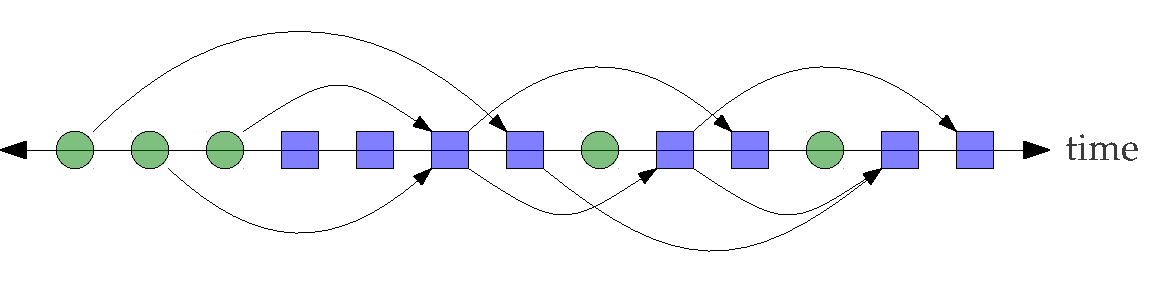
\includegraphics[width=10cm]{gfx/dependency_traces}
%% %\caption{Dependency traces as propagator cells.}
%% %\label{figure:propogators_dependency_traces}
%% %\end{figure}

